\section{Zweidimensionale Richtungsbestimmung} \todo{Durchlesen + überprüfen}
\subsection{Erweiterung der Theorie}
Um die eindimensionale Richtungsbestimmung auf den zweidimensionalen Raum zu erweitern, muss man lediglich $s_y$ nicht mehr als konstant betrachten. Dadurch hat die Gleichung, die für das Eindimensionale eindeutig war, nun zwei Unbekannte: $s_x$ und $s_y$. Um im Zweidimensionalen eine Ortung durchzuführen, wird deswegen ein drittes Mikrofon $M_3$ benötigt. Auch der Abstand zwischen dem dritten Mikrofon und dem ersten darf maximal so groß wie die Wellenlänge sein. Mit dem drittem Mikrofon kann eine weitere Gleichung, die den Gangunterschied zwischen dem ersten und dem dritten Mikrofon $\Delta{x_{13}}$ enthält, aufgestellt werden. Man erhält das Gleichungssystem:
$$\begin{cases}
  \abs{\vec{m}_1 - \vec{s}} - \abs{\vec{m}_2 - \vec{s}} = \Delta{x_{12}} \\
  \abs{\vec{m}_1 - \vec{s}} - \abs{\vec{m}_3 - \vec{s}} = \Delta{x_{13}}
\end{cases}$$
$$\begin{cases}
  \sqrt{{(m_{1_x} - s_x)}^2 + {(m_{1_y} - s_y)}^2} - \sqrt{{(m_{2_x} - s_x)}^2 + {(m_{2_y} - s_y)}^2} = \Delta{x_{12}} \\
  \sqrt{{(m_{1_x} - s_x)}^2 + {(m_{1_y} - s_y)}^2} - \sqrt{{(m_{3_x} - s_x)}^2 + {(m_{3_y} - s_y)}^2} = \Delta{x_{13}}
\end{cases}$$
Graphisch veranschaulicht entspricht dieses Gleichungssystem der Suche nach dem Schnittpunkt von zwei halben Hyperbeln um zwei der Mikrofone
\begin{figure}[H]
  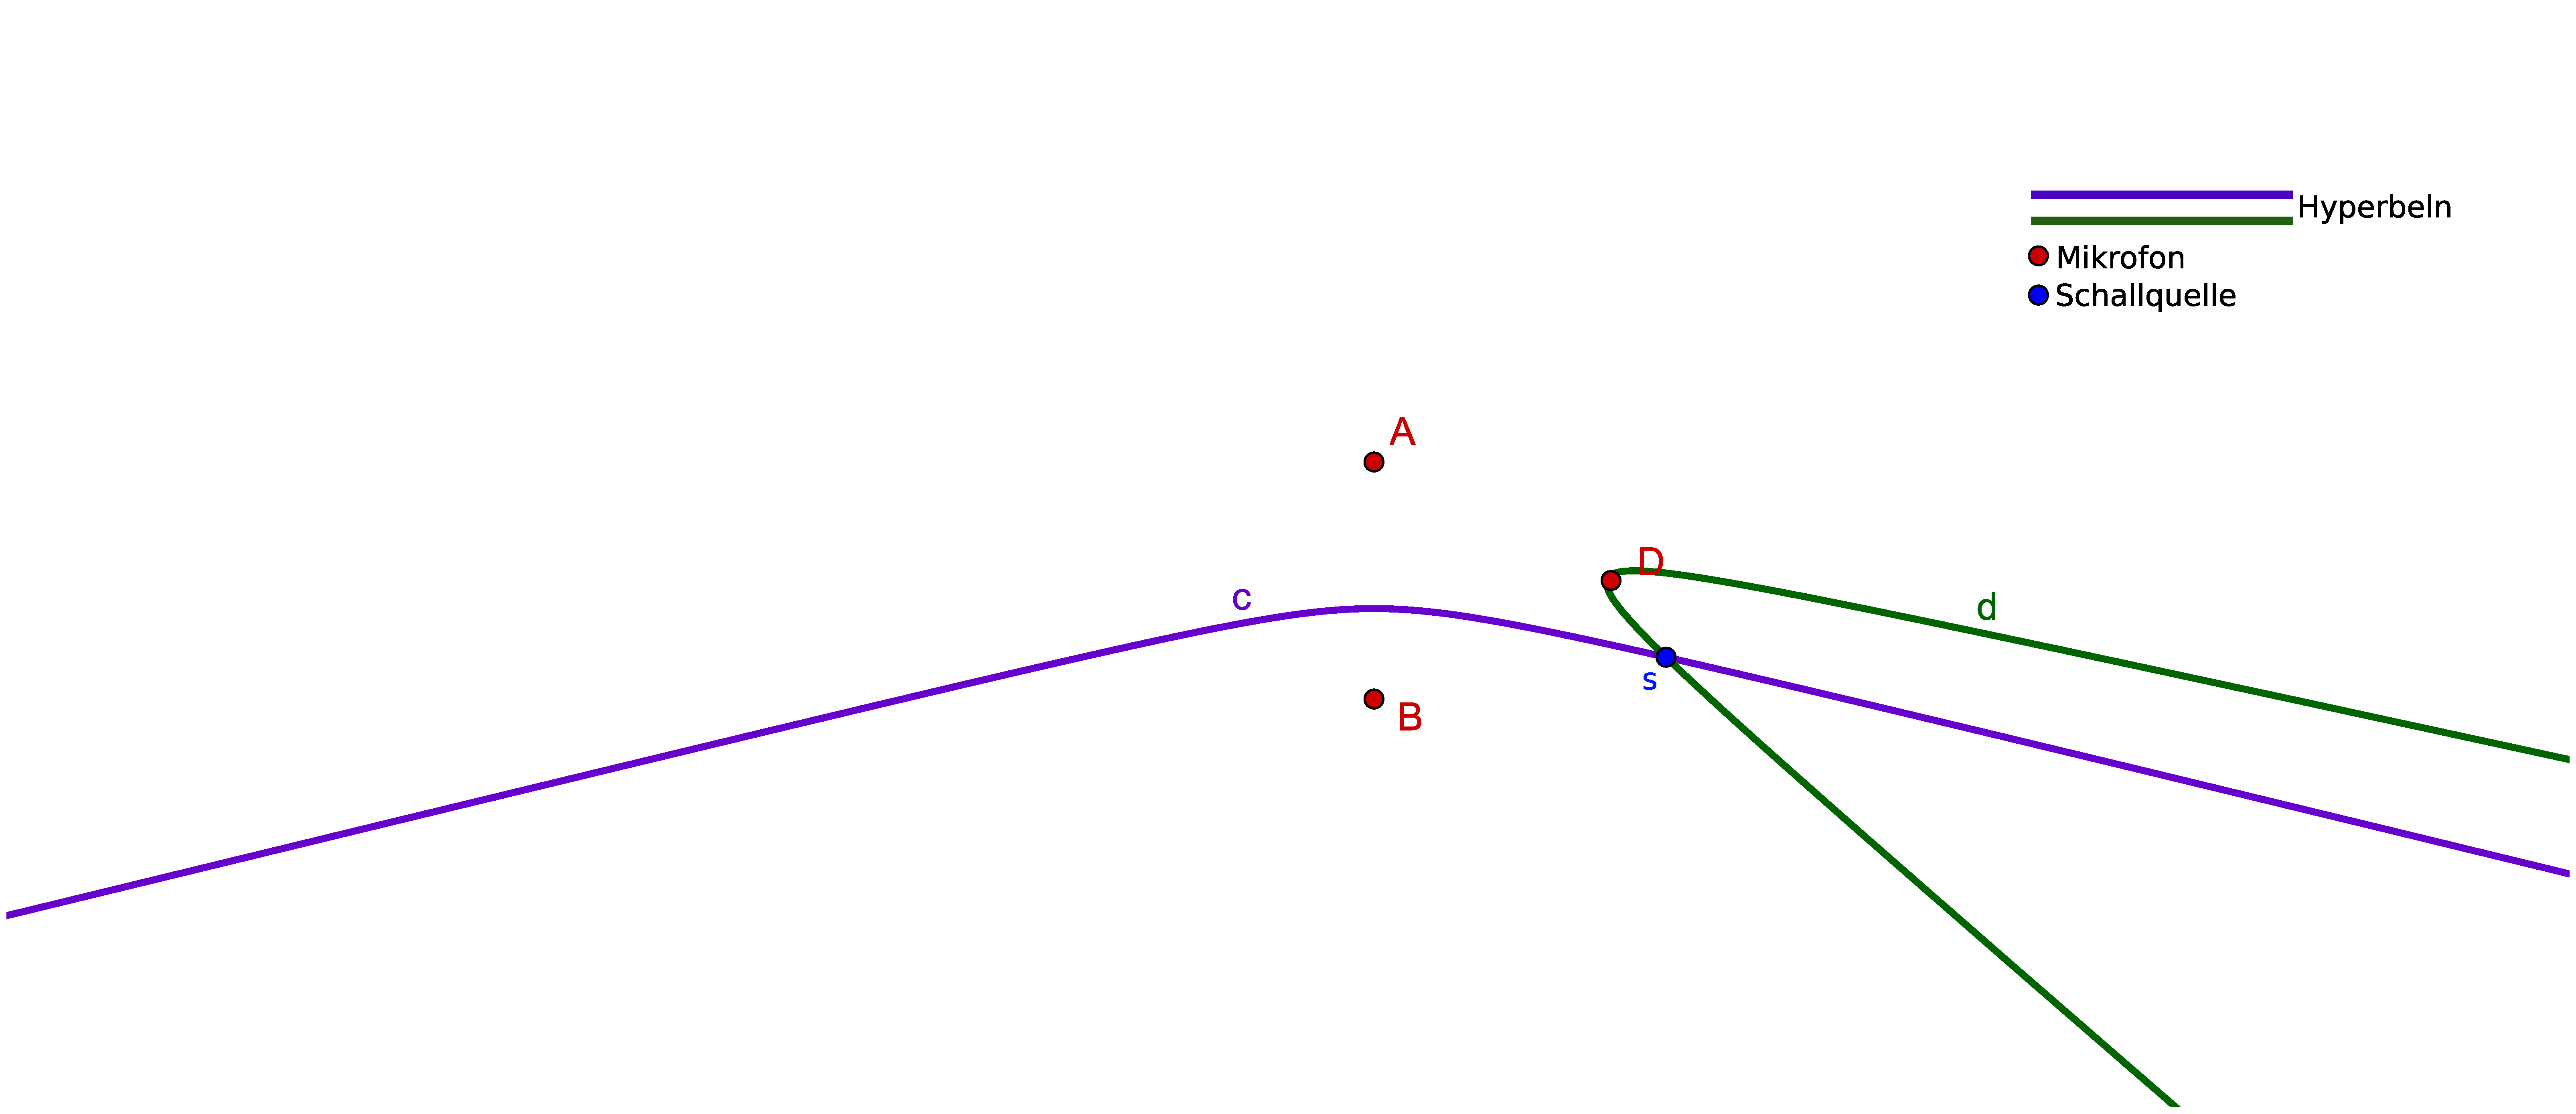
\includegraphics[width=\linewidth]{img/skizze1d}
  \caption{Veranschaulichung des Gleichungssystems durch den Schnittpunkt von zwei Hyperbeln, die roten Punkte stellen die Mikrofone dar und der grüne Punkt die Schallquelle}
\end{figure}

\subsection{Analytische Lösung des Gleichungssystems}
Dieses Gleichungssystem haben wir mit Hilfe des Computer Algebra Systems \textit{Wolfram Mathematica}\cite{mathematica} nach $\vec{s}$ aufgelöst:
\begin{lstlisting}[language=Mathematica,caption={Befehl um das Gleichungssystem in \textit{Mathematica} zu lösen}]
  Solve[{
    Sqrt[(m1x - sx)^2 + (m1y - sy)^2] - Sqrt[(m2x - sx)^2 + (m2y - sy)^2] = dx12,
    Sqrt[(m1x - sx)^2 + (m1y - sy)^2] - Sqrt[(m3x - sx)^2 + (m3y - sy)^2] = dx13,}
  {sx, sy}]
\end{lstlisting}
Da das Gleichungssystem nicht linear ist, ist die Lösung sehr kompliziert, gedruckt entspricht sie fünf Seiten. \textit{Mathematica} findet für dieses Gleichungssystem außerdem zwei allgemeine reelle Lösungen, man erhält also zwei mögliche Richtungen.
